\documentclass[a4paper]{article}

  \usepackage{fullpage} % Package to use full page
  \usepackage{parskip} % Package to tweak paragraph skipping
  \usepackage{tikz} % Package for drawing
  \usepackage{amsmath}
  \usepackage{siunitx} % Package for scientific units
  \usepackage{amsfonts}
  \usepackage{amssymb}
  \usepackage{hyperref}
  \usepackage[utf8]{inputenc}
  \usepackage[english]{babel}
  \usepackage{multicol}
  \usepackage{graphicx} % Package for including images
  \graphicspath{ {./images/} }
  
  \newcommand\tab[1][0.5cm]{\hspace*{#1}}
  
  \title{Lab 2}
  \author{Adrian Darian}
  \date{9/14/2020}
  
  \begin{document}
  
\maketitle
  
\section*{Discussion Section 2}

\section*{Instructions:}
This week you will compute questions involving the normal distribution. You will receive some basic guidance in R from your TAs and a piece of code that you may find helpful in
completing your work. You are welcome to work alone or in small groups but everyone is responsible for turning in their own code/assignment.

This week, you are responsible for submitting \textbf{only} a written report. (No code is required in the submission!) However, your report must include for each problem below:

\begin{itemize}
    \item A picture indicating the region of the domain the problem is referring to. (See the examples on each slide.)
    \item The numerical solution to each problem below.
\end{itemize}

As in all written work, you must use complete sentences and explain your reasoning. Simply providing the correct answer, without justification, is not considered complete.

\section*{Assignment:}
You will answer the following three questions either using the pnorm function in R which determines the cumulative distribution for the Normal Random Variable or using another online tool such as http://onlinestatbook.com/2/calculators/normal.html. For each case you must responsible for submitting a picture (which shows normal PDF shaded with the area you want to calculate.)

\begin{itemize}
    \item[1.] (2 Points): Let $X$ be a normally distributed random variable with mean $u = 29$ and $o^2 = 6$. Determine the probability that $X$ is larger than $35$. \\
    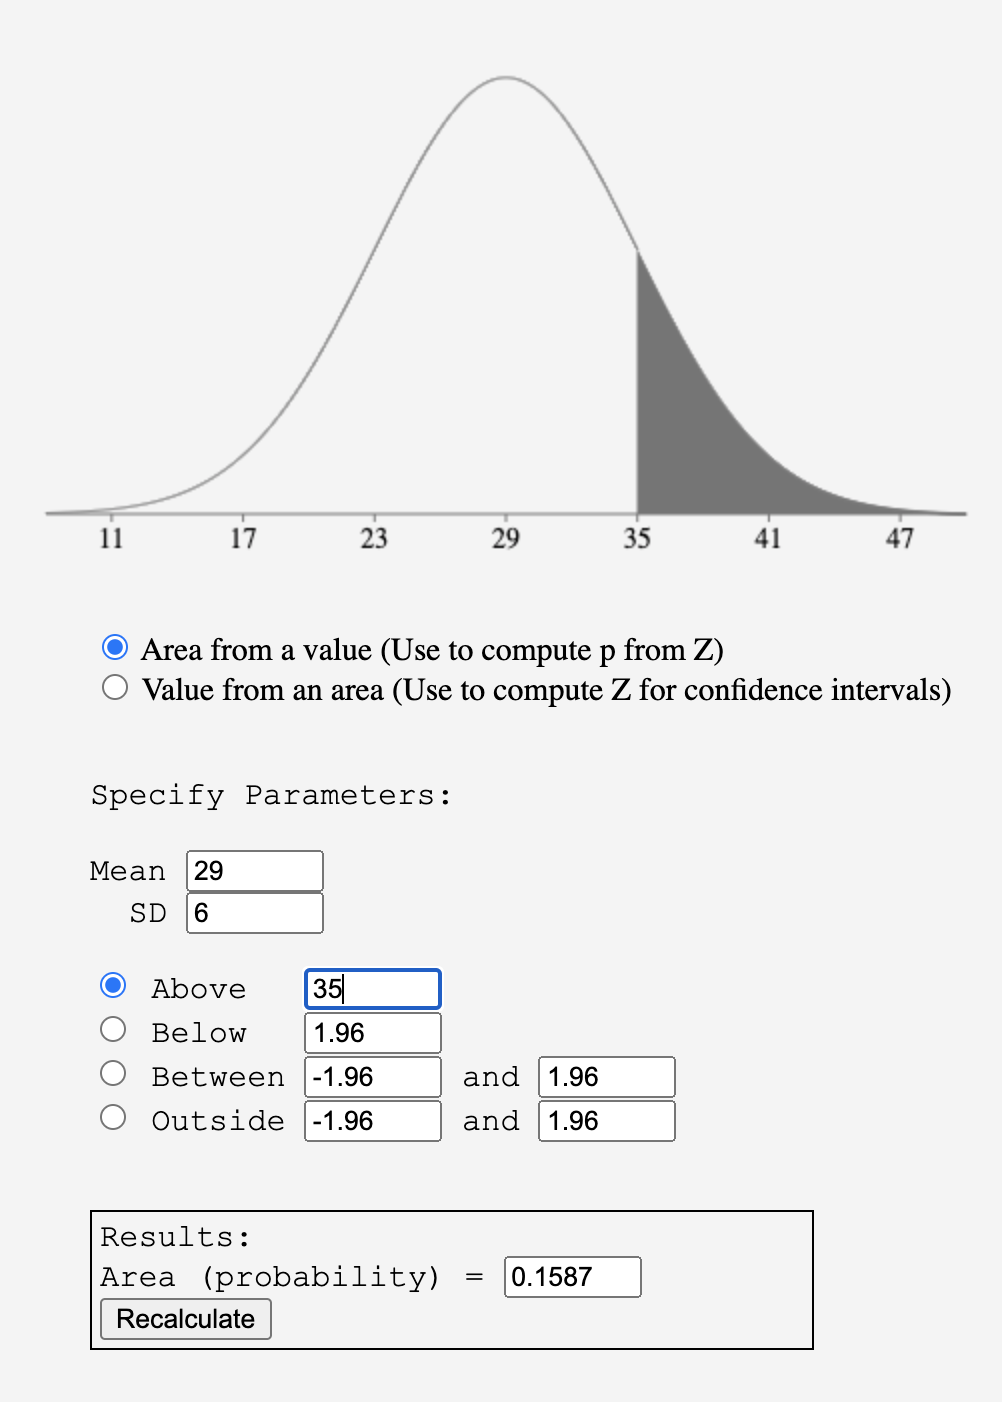
\includegraphics[scale=0.5]{Question-1.png} 
    \item[2.] (2 Points): Let $X$ be a normally distributed random variable with mean $u = 5$ and $o^2 = 10$. Determine the probability that $X$ is smaller than $4$. \\
    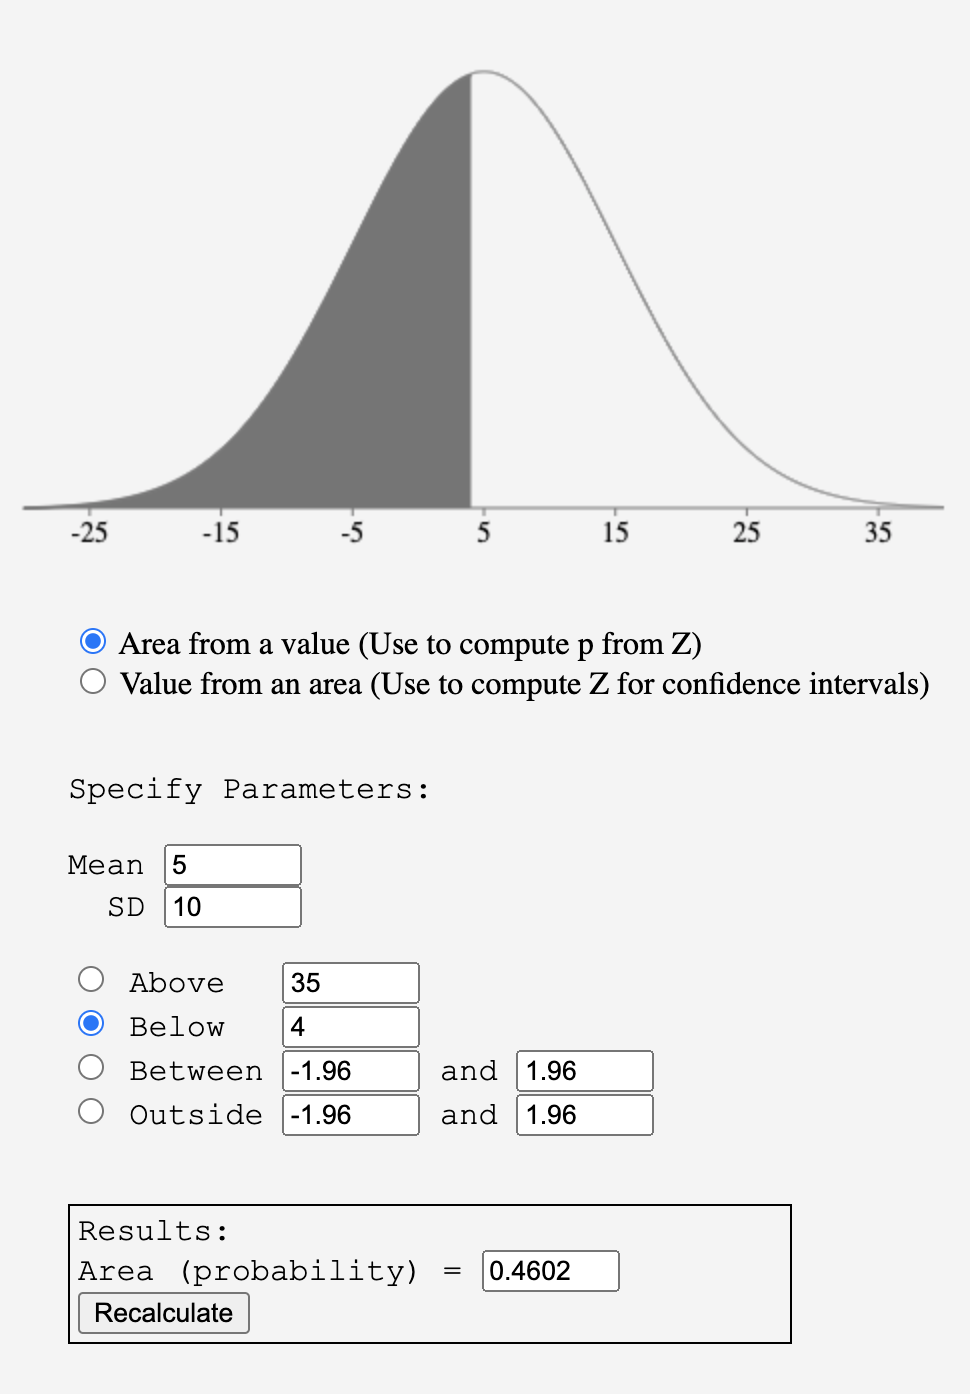
\includegraphics[scale=0.5]{Question-2.png}  
    \item[3.] (2 Points): Let $X$ be a normally distributed random variable with mean $u = 20$ and $o^2 = 36$. Determine the probability that $X$ is between $16.2$ and $27.5$. \\
    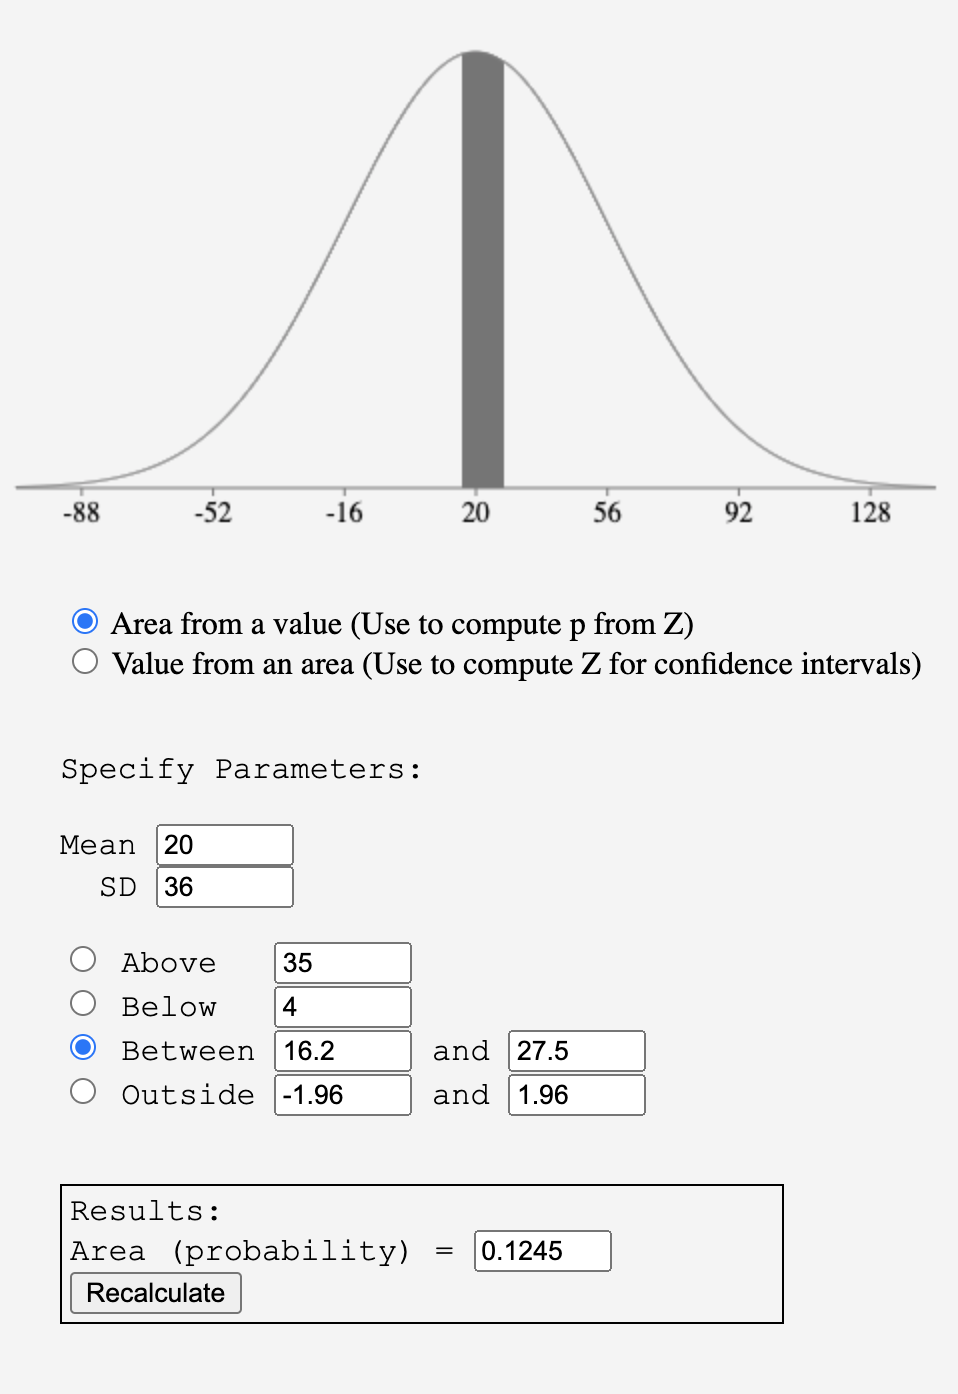
\includegraphics[scale=0.5]{Question-3.png}  
    \item[4.] (2 Points:) Let $X$ be a normally distributed random variable with mean $u = 0$ for what standard deviation will $P(-5 \leq X \leq 5) = 0.5$. (Hint: One solution to this problem is to modify the R code “Lab05 ClassExample.R” you were given. The range of σ you should consider will need to be changed as well different.) \\
    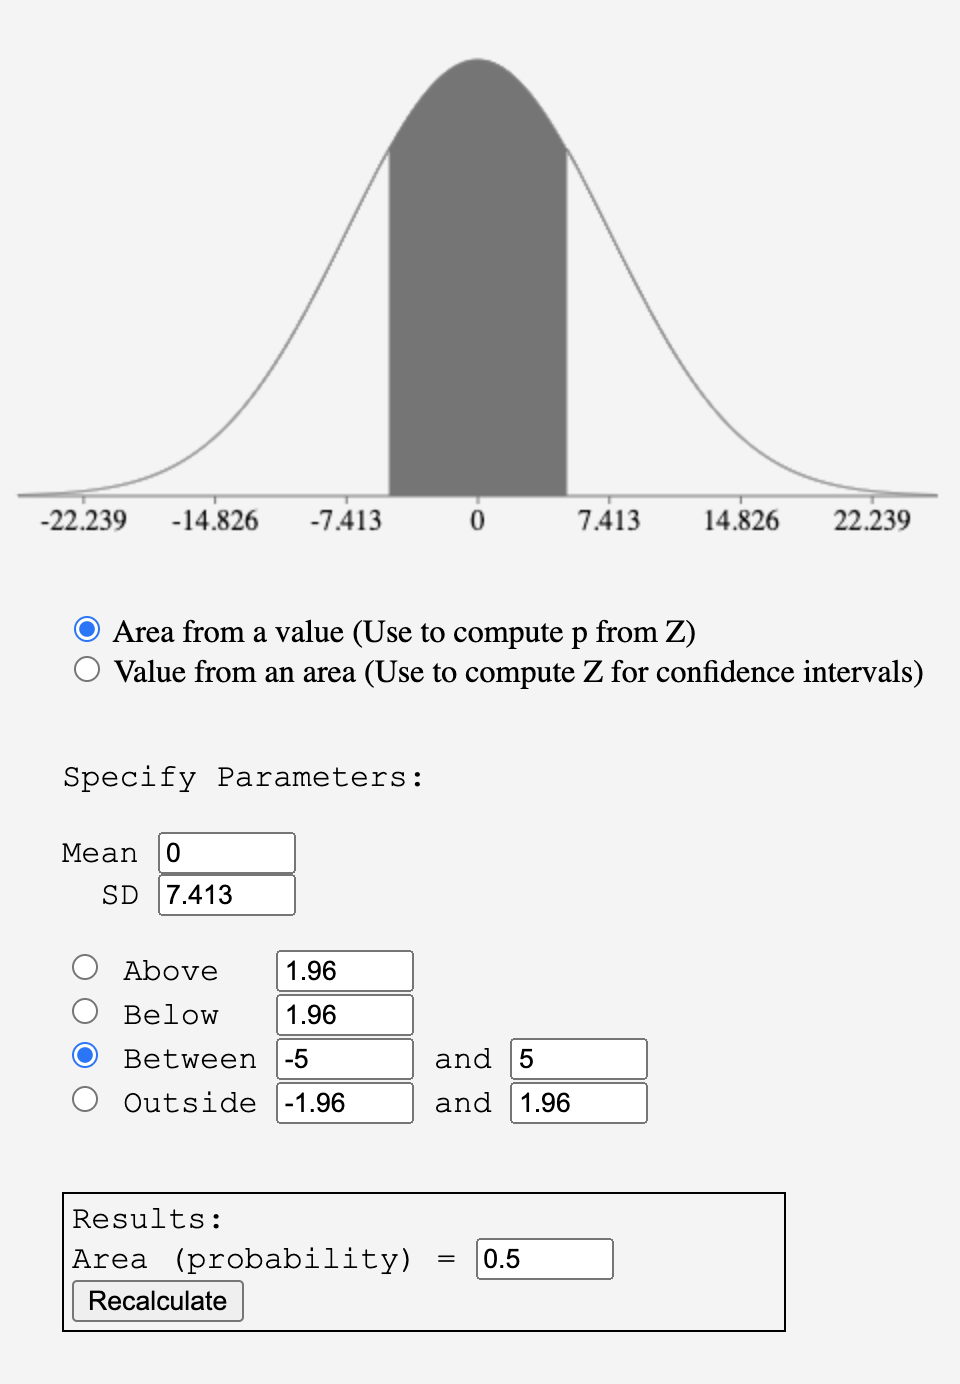
\includegraphics[scale=0.5]{Question-4.png}
    \item[5.] (2 Points:) A machine that produces ball bearings has been set so that the true average diameter of the bearings is produces is $0.500$ inches. A bearing is acceptable if its diameter is within $0.004$ inches of this target value. Suppose, however, that the machine setting has been changed during the course of production. The diameter of ball bearings produced by this new setting have been verified to follow a normal distribution with mean value $0.499$ inches and a standard deviation of $0.002$ inches. \\
    What percentage of the bearings produced will be unacceptable? \\
    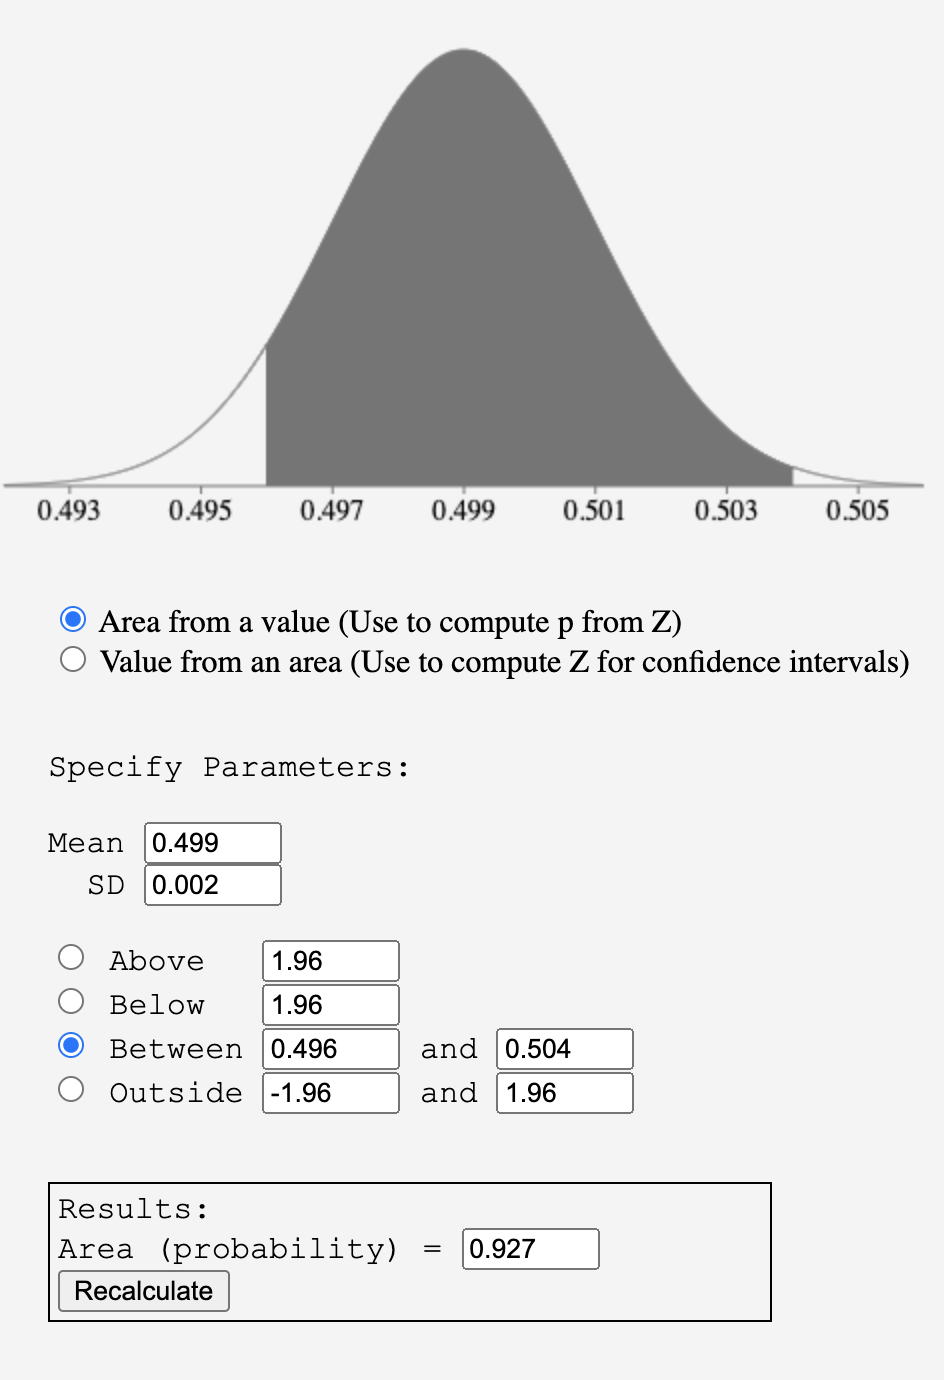
\includegraphics[scale=0.5]{Question-5.png}
\end{itemize}
  
\end{document}